\section*{\centering{Summary of April 13, 2016 phone conference and requests from the NP-PWG review committee
M. Garcon, S. Kuhn and Zein-Eddine Meziani\\ 
to M. Hattawi and co-authors}}

\begin{enumerate}
\item RTPC calibration: all previous questions are considered answered 
satisfactorily. Remains a significant effort to rewrite the corresponding 
section(s) more clearly.

\item Event selection cuts: the committee acknowledges the numerous studies 
(variation of cuts) that have been performed. It is not fully convinced, 
however, that there is no remaining background (other than $\pi^{0}$s only) in 
either channel, and about the argument on the statistics (for cutting tails).  
Consequently, it is requested:
\begin{enumerate}
\item To show plots of correlations between exclusivity cuts:
\begin{enumerate}
  \item 2D missing $ep\gamma X$ M2 vs $\Delta \phi$: is there a gain to be 
     expected by a contour cut? If yes, implement. Shown in figure 
     \ref{fig:2d_delta_phi_MM2_InCoh}
    \begin{figure}[!h]
    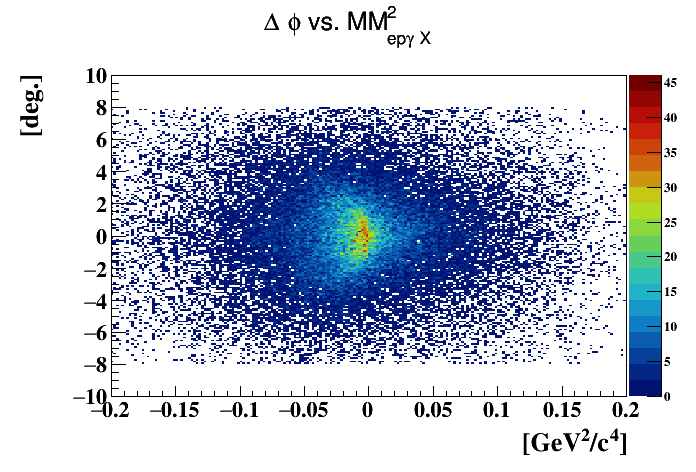
\includegraphics[height=5.6cm]{fig/delta_phi_epgamma_M2_Mis.png}
    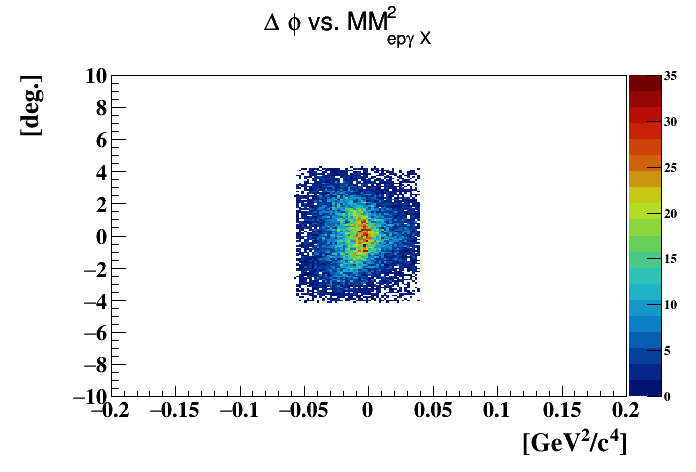
\includegraphics[height=5.6cm]{fig/delta_phi_epgamma_M2_Mis_with.png}
    \caption{ $\Delta \phi$ vs. $MM^{2}_{ep\gamma X}$ before (left) and 
    after (right) the exclusivity cuts.}
    \label{fig:2d_delta_phi_MM2_InCoh}
    \end{figure}                                                                  


  \item Produce all 9 plots in right figure of slides 5 and 9 of \url{ 
     https://clasweb.jlab.org/rungroups/lowq/wiki/images/a/a0/ExcluCuts-CANeg6.pdf}   
     for a 2$\sigma$ and 1$\sigma$ cuts on missing $ep\gamma X$ M2.
    \begin{figure}[tbp]
    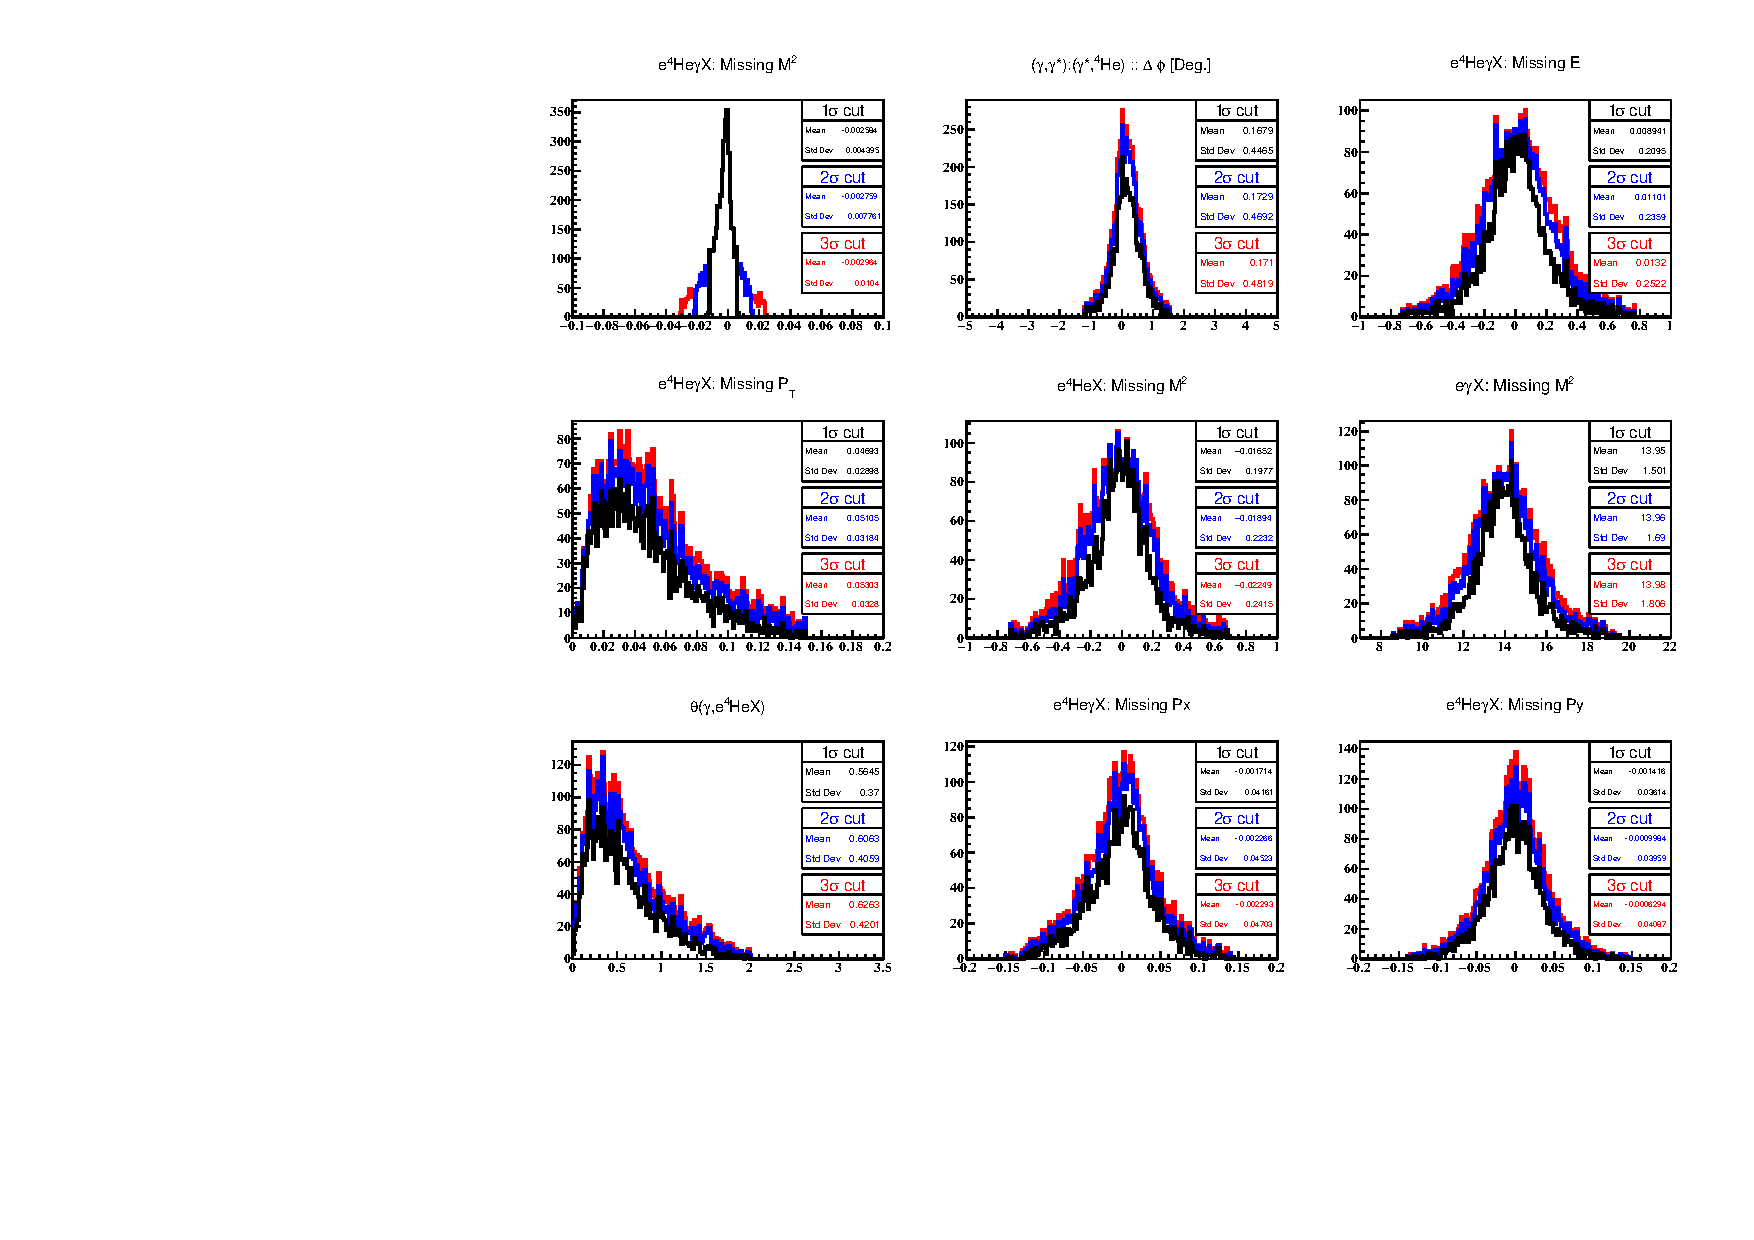
\includegraphics[height=14.6cm]{fig/all_sigmas_coh_exc_cuts.pdf}
    \caption{Coherent exclusivity distributions for the different cut 
    width on $e^{4}He\gamma X$ missing mass squared. }
    \label{fig:2d_delta_phi_MM2_InCoh}
    \end{figure}                                                                  
    \begin{figure}[tbp]
    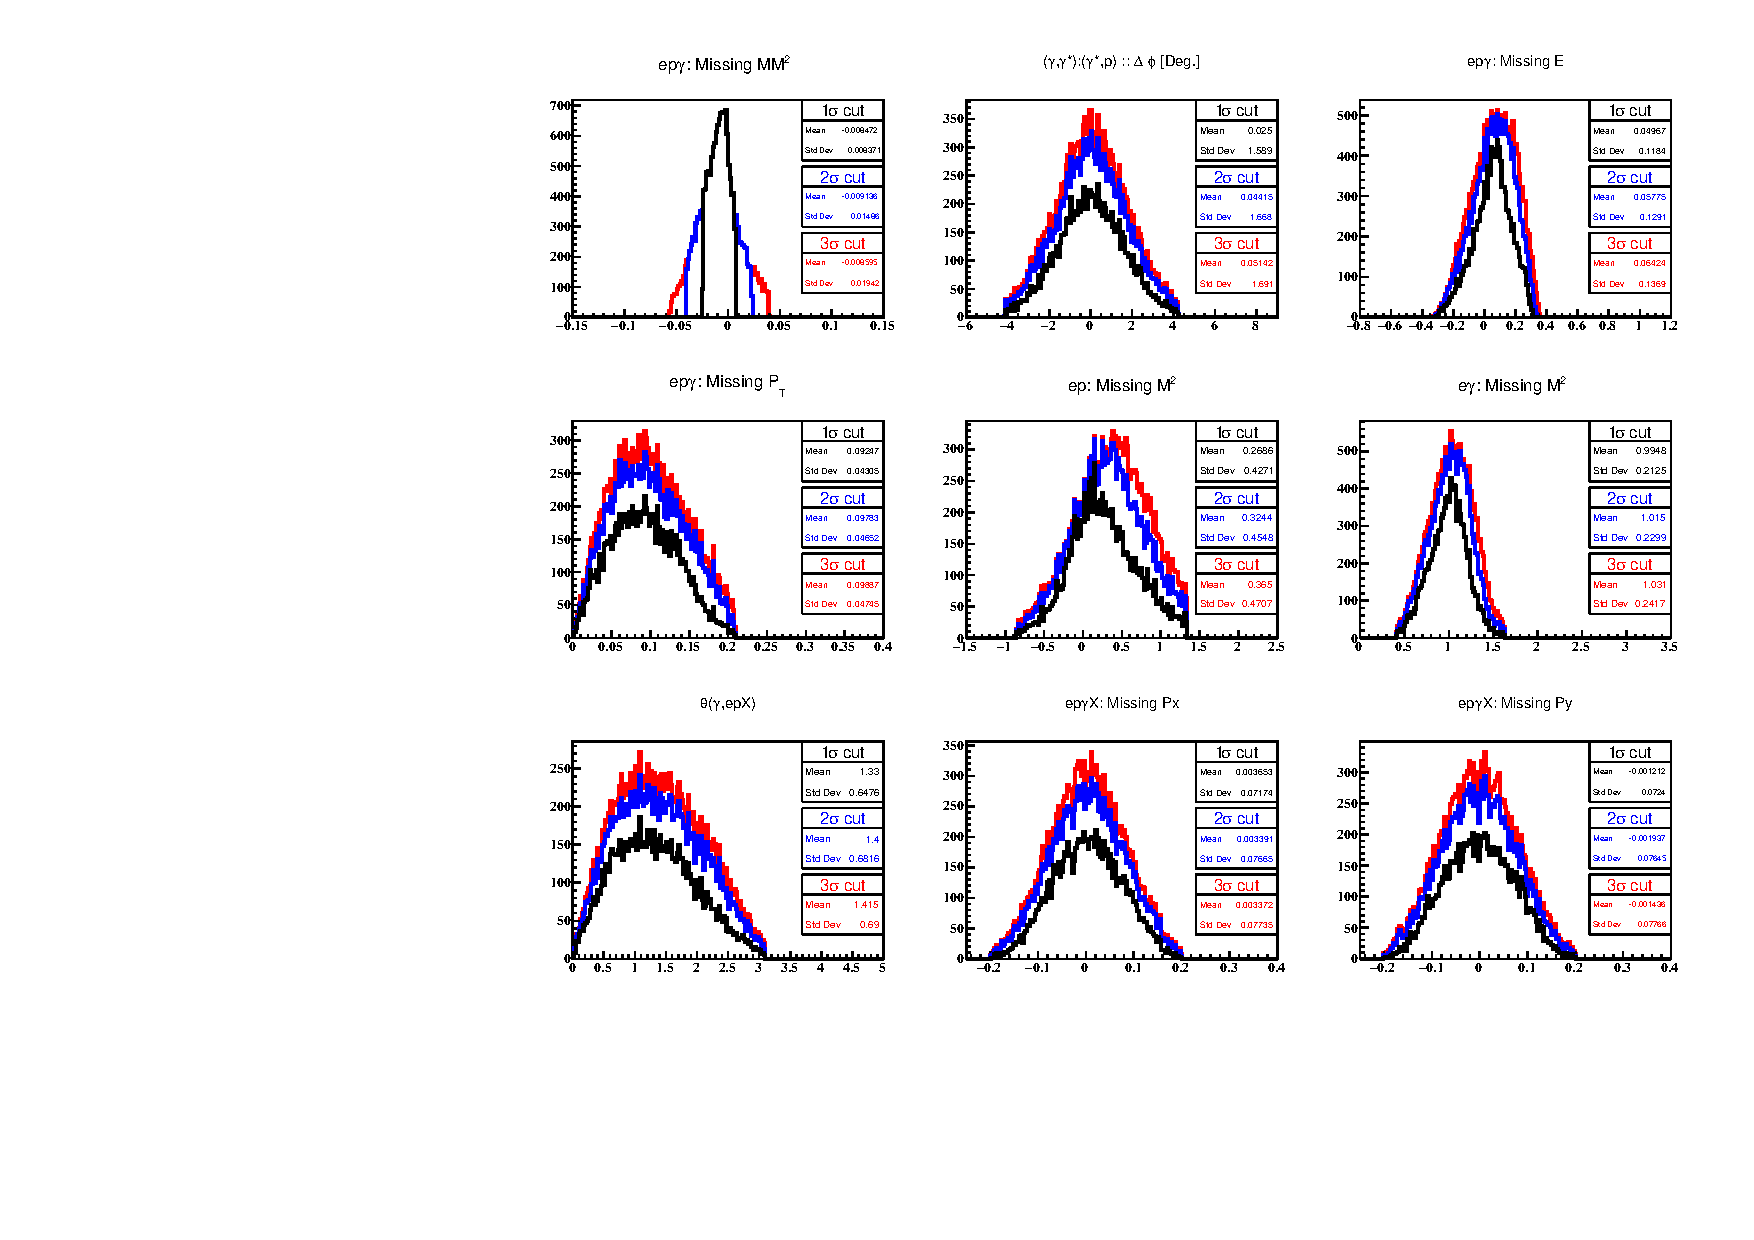
\includegraphics[height=14.6cm]{fig/all_sigmas_incoh_exc_cuts.pdf}
    \caption{ Incoherent exclusivity distributions for the different cut  
    width on $ep\gamma X$ missing mass squared.}
    \label{fig:2d_delta_phi_MM2_InCoh}
    \end{figure}                                                                  



    \end{enumerate}
\item (optionally) In the incoherent case, extract ALU with 2 variations of the 
   ep missing M2 right cut, moving it tighter to the left (e.g.  1 and 0.75 
   GeV2).  (also see the evolution of the other distributions when doing so).
\end{enumerate}

\item Free proton asymmetries from FX's publication: implement a (possibly 3D/9 
points) interpolation to smooth out both statistical fluctuations and 
kinematical dependences. Reintroduce a corresponding section in the CAN. Take 
into account both stat. and syst. errors of both experiments in the ratio. The 
committee recommends though to be cautious about the statements on the 
asymmetry ratios in the future publication.

\item CFF: the committee acknowledges that the new procedure (2-parameter fit 
with complete formula at leading-twist) is more satisfying. It recommends 
though to be cautious about the statements on CFF in the future publication.

\item CAN: a number of answers to previous questions have to appear in the CAN.  
This includes (but may not be limited to) 

Figs 1-4 of \url{https://clasweb.jlab.org/rungroups/lowq/wiki/images/a/a3/Final_1st_round_comments.pdf} 
Tighter $edist$ cut [-2,+3 mm].
Otherwise, even if you do not show it in the CAN, mention in one line that a 
specific study was done.
\item Miscellaneous:
   \begin{enumerate}
      \item 4-D dependences of the ratio R: the statement that the integrated R's 
    are flat is disputable (see Figs 4.16 and 4.17), but we are ready to accept 
    that the effect discussed is small and taken care of in the systematic 
    errors.
 \item not convinced that comparing 9 phi-bins to 11 is a definitive answer, 
    when not applying any finite bin size correction. But again, in view of the 
    size of statistical and systematic errors, would accept that.
 \item Your Eq.(4) of "answer" is probably wrong. For our own understanding, 
   look into this argument again.
\item ...
   \end{enumerate}

\item Please keep a record of the changes in the CAN, as we will probably not 
re-read the whole text.

\item Request to see the very first draft of the publication.
\end{enumerate}
